\section{Introdução}

\subsection{Cálculo do $\pi$? Black-Scholes?}

Este trabalho implementa algoritmos conhecidos para o cálculo de muitas casas decimais do número $\pi$. O objetivo com isso não é obter uma precisão gigantesca e inútil do número $\pi$, mas sim aplicar conhecimentos da disciplina de Programação Concorrente nos algoritmos implementados. Para isso é feita a implementação sequencial e paralela (\emph{multi-thread}) de cada algoritmo, e são eles: Gauss-Legendre \cite{gauss-legendre}, Borwein (1984) \cite{borwein} e Método de Monte Carlo \cite{monte-carlo}.

Além disso, este trabalho também implementa as versões sequencial e paralela da Simulação Monte Carlo para o algoritmo de Black-Scholes \cite{bs} que descreve um fenômeno financeiro que é a precificação de derivativos. O algoritmo implementado é o descrito na especificação do trabalho.

Este relatório faz parte de um conjunto de arquivos referentes ao trabalho. A documentação do código-fonte encontra-se nos próprios arquivos \texttt{.c} referentes aos algoritmos dentro do diretório \texttt{./src} a partir do diretório raiz.

\subsection{Os Algoritmos}

\subsubsection{Gauss-Legendre}

O algoritmo de Guass-Legendre é um algoritmo para computar os dígitos do $\pi$ e é notável por sua convergência quadrática.

\begin{algorithm}[H]
	\begin{enumerate}

		\item Define-se os valores iniciais para as variáveis:
		$$
			a_0 = 1 \quad, \quad b_0 = \frac{1}{\sqrt{2}} \quad, \quad t_0 = \frac{1}{4} \quad, \quad p_0 = 1
		$$

		\item Repete-se os seguintes passos até que a diferença entre $a_n$ e $b_n$
		esteja dentro da precisão desejada:
			\begin{align}
				a_{n+1} & = \frac{a_n + b_n}{2}               \label{eq:gs-1} \\[1em]
				b_{n+1} & = \sqrt{a_n \cdot b_n}              \label{eq:gs-2} \\[1em]
				t_{n+1} & = t_n - p_n \cdot (a_n - a_{n+1})^2 \label{eq:gs-3} \\[1em]
				p_{n+1} & = 2 \cdot p_n                       \label{eq:gs-4}
			\end{align}

		\item Obtém-se $\pi$ aproximando por:
			\begin{align}
				\pi \approx \frac{(a_{n+1} + b_{n+1})^2}{4 \cdot t_{n+1}}  \label{eq:gs-5}
			\end{align}

	\end{enumerate}
\caption{Gauss-Legendre \label{alg:gs}}
\end{algorithm}

\subsubsection{Borwein (1984)}

Este algoritmo de Borwein é um dos usados para se calcular dígitos do $\pi$ e também possui convergência quadrática.

\begin{algorithm}[H]
	\begin{enumerate}

		\item Define-se os valores iniciais para as variáveis:
			$$
				a_0 = \sqrt{2} \quad, \quad b_0 = 0 \quad, \quad p_0 = 2 + \sqrt{2}
			$$

		\item Repete-se os seguintes passos até que $p_n$ aproxime $\pi$ na quantidade
		de dígitos desejada:
			\begin{align}
				a_{n+1} & = \frac{a_n + 1}{2 \cdot \sqrt{a_n}}                        \label{eq:b-1} \\[1em]
				b_{n+1} & = \frac{(1 + b_n) \cdot \sqrt{a_n}}{a_n + b_n}              \label{eq:b-2} \\[1em]
				p_{n+1} & = \frac{(1 + a_{n+1}) \cdot p_n \cdot b_{n+1}}{1 + b_{n+1}} \label{eq:b-3}
			\end{align}

		\item Obtém-se $\pi$ aproximando por:
			\begin{align}
				\pi \approx p_n    \label{eq:b-4}
			\end{align}
	\end{enumerate}
\caption{Borwein (1984) \label{alg:borwein}}
\end{algorithm}

\subsubsection{Método de Monte Carlo}

O Método de Monte Carlo para o cálculo $\pi$ consiste em:

\begin{figure}[h]
\centering
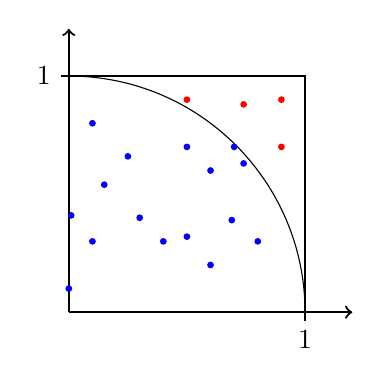
\begin{tikzpicture}[scale=0.3em]
	\draw[thick,->] (0,0) -- (1.2,0);
	\draw[thick,->] (0,0) -- (0,1.2);

	\draw (0,0) -- (1,0) -- (1,1) -- (0,1) -- (0,0);
	\draw (1,0) arc (0:90:1);

	\draw (1,1pt) -- (1,-1pt) node[anchor=north] {$1$};
	\draw (1pt,1) -- (-1pt,1) node[anchor=east] {$1$};

	\node[color=blue, mark size=1pt] at (0.8, 0.3) {\pgfuseplotmark{*}};
	\node[color=blue, mark size=1pt] at (0.5, 0.7) {\pgfuseplotmark{*}};
	\node[color=blue, mark size=1pt] at (0.6, 0.6) {\pgfuseplotmark{*}};
	\node[color=blue, mark size=1pt] at (0.4, 0.3) {\pgfuseplotmark{*}};
	\node[color=blue, mark size=1pt] at (0.7, 0.7) {\pgfuseplotmark{*}};
	\node[color=blue, mark size=1pt] at (0.6, 0.2) {\pgfuseplotmark{*}};
	\node[color=blue, mark size=1pt] at (0.1, 0.3) {\pgfuseplotmark{*}};
	\node[color=blue, mark size=1pt] at (0.0, 0.1) {\pgfuseplotmark{*}};
	\node[color=blue, mark size=1pt] at (0.69, 0.39) {\pgfuseplotmark{*}};
	\node[color=blue, mark size=1pt] at (0.3, 0.4) {\pgfuseplotmark{*}};
	\node[color=blue, mark size=1pt] at (0.1, 0.8) {\pgfuseplotmark{*}};
	\node[color=blue, mark size=1pt] at (0.25, 0.66) {\pgfuseplotmark{*}};
	\node[color=blue, mark size=1pt] at (0.15, 0.54) {\pgfuseplotmark{*}};
	\node[color=blue, mark size=1pt] at (0.5, 0.32) {\pgfuseplotmark{*}};
	\node[color=blue, mark size=1pt] at (0.01, 0.41) {\pgfuseplotmark{*}};
	\node[color=blue, mark size=1pt] at (0.74, 0.63) {\pgfuseplotmark{*}};

	\node[color=red, mark size=1pt] at (0.9, 0.9) {\pgfuseplotmark{*}};
	\node[color=red, mark size=1pt] at (0.74, 0.88) {\pgfuseplotmark{*}};
	\node[color=red, mark size=1pt] at (0.9, 0.7) {\pgfuseplotmark{*}};
	\node[color=red, mark size=1pt] at (0.5, 0.9) {\pgfuseplotmark{*}};

\end{tikzpicture}
\caption{Ilustração do algoritmo para cálculo do $\pi$ com Método Monte Carlo. \label{fig:mc-img}}
\end{figure}

\begin{algorithm}[H]
	\begin{enumerate}
		\item Toma-se um quadrado de lado $l = 1$ e dentro dele um setor de $90\degree$ de raio $r = 1$.

		\item Gera-se aleatoriamente $N$ pontos $(x, y) \in [0, 1]$

		\item Então, para cada um dos $N$ pontos, confere se:
		$$
			x^2 + y^2 \leq 1
		$$

		\item Conta-se em $C$ quantos pontos satisfazem a condição acima

		\item Obtém-se $\pi$ aproximando por:
		$$
			\pi \approx \frac{4 \cdot C}{N}
		$$
	\end{enumerate}
\caption{Método Monte Carlo para $\pi$ \label{alg:mc}}
\end{algorithm}

\subsubsection{Black-Scholes}

Foi elaborado por dois cientistas chamados Fisher Black e Myron Scholes, que adaptaram uma fórmula física para descrever um fenômeno financeiro que é a precificação de derivativos.

\begin{algorithm}[H]
\Indm\Indp
	\BlankLine
	\SetKwFunction{randomNumber}{randomNumber}
	\SetKwFunction{max}{max}
	\SetKwFunction{mean}{mean}
	\SetKwFunction{stddev}{stddev}
	\SetKwFunction{exp}{exp}

	$S \leftarrow$ \text{valor da ação} \\
	$E \leftarrow$ \text{preço de exercício da opção} \\
	$r \leftarrow$ \text{taxa de juros livre de risco (SELIC)} \\
	$\sigma \leftarrow$ \text{volatilidade da ação} \\
	$T \leftarrow$ \text{tempo de validade da opção} \\
	$M \leftarrow$ \text{número de iterações}
	\BlankLine

	\For{$i\leftarrow 0$ \KwTo $M-1$}{
		$t \leftarrow S \cdot \exp((r-0.5 \cdot \sigma^2) \cdot T + \sigma\sqrt{T}\cdot\randomNumber())$ \\
		$trials[i] \leftarrow \exp(-r \cdot T) \cdot \max(t-E, 0)$ \\
	}
	\BlankLine

	$mean \leftarrow \mean(trials)$\\
	$stddev \leftarrow \stddev(trials, mean)$\\
	$confwidth \leftarrow 1.96 \cdot stddev / \sqrt{M}$\\
	$confmin \leftarrow mean - confwidth$\\
	$confmax \leftarrow mean + confwidth$\\
	\BlankLine
	\BlankLine
	\BlankLine

\caption{Black-Scholes \label{alg:bs}}
\end{algorithm}

